\documentclass[letterpaper]{article}

 \usepackage{amsmath}
\usepackage[utf8]{inputenc}
\usepackage[T1]{fontenc}
\usepackage{lmodern} % load a font with all the characters
\usepackage[utf8]{inputenc}
 \usepackage[pdftex]{graphicx}

\begin{document}

\title{Distributed HMM}
\author{Megha Gupta}
\maketitle
\section{Automata and their products}
\label{sec:intro}

Distributed networks can be modelled using interacting automata. Benveniste defines automaton as a quadruple, \'{A} = (X,X$_{0}$,A,T) where X is a finite state of sets, X0 is the subset of initial states, A is a finite set of messages, T is a set of transitions of the form t = \{x\_,a,x\} where x\_ is the previous state, a is the message label on which the state transitions to the next state x. The figure~\ref{fig:ex} below explains the automata with an example.\\

\begin{figure*}[t]
\centering
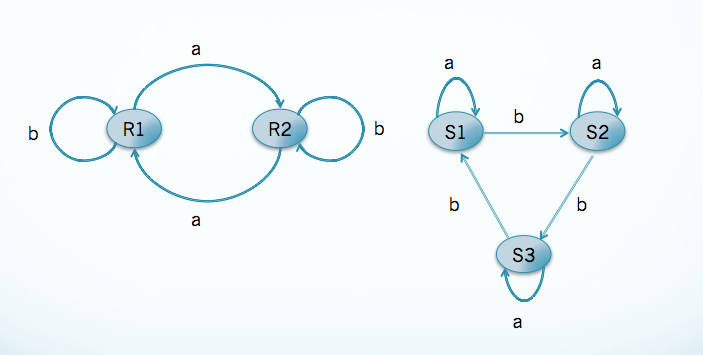
\includegraphics[width=10cm,height=5cm]{automata.png}
\caption{Automata R and S}
\label{fig:ex}
\end{figure*}

For automaton R, X$_{R}$ = \{2; R1,R2\}, X$_{0R}$ = \{R1\}, A$_{R}$ = \{a,b\}, T$_{R}$ = \{R1,a,R1; R1,b,R2; R2,a,R2; R2,b,R1\} \\
For automaton S, X$_{S}$ = \{3; S1,S2,S3\}, X$_{0S}$ = \{S1\}, A$_{S}$ = \{a,b\}, T$_{S}$ = \{S1,a,S1; S1,b,S2; S2,a,S2; S2,b,S3; S3,a,S3; S3,b,S1\} \\
The product of two automata \'{A} = R x S is defined as follows: \\
X = X$_{R}$ x X$_{S}$ \\
X$_{0}$ = X$_{0R}$ x X$_{0S}$ \\
A = A$_{R}$ $\cup$ A$_{S}$ \\
%t = (x\_,a,x)  \\
Benveniste uses a notion of stuttering transition which helps to distinguish between local and global time by inserting dummy transitions between two transitions of a local automaton attached to a node. This stuttering transition does nothing but lets the rest of the world progress.

\begin{table}[h]
\centering
\begin{tabular}{ l | c | c }
 A & R1 & R2 \\
\hline
R1 & 0.6 & 0.4 \\
R2 & 0.3 & 0.7 \\
\end{tabular}
\caption{Transition probability, A}
\label{table:A}
\end{table}

\begin{table}[h]
\centering
\begin{tabular}{ l | c | c }
 B & a & b \\
\hline
R1 & 0.2 & 0.8 \\
R2 & 0.5 & 0.5 \\
\end{tabular}
\caption{Observed probability, B}
\label{table:B}
\end{table}

\begin{table}[h]
\centering
\begin{tabular}{ l | c | c }
&  R1 & R2 \\
\hline
$\pi$ & 0.4 & 0.6 \\

\end{tabular}
\caption{Initial state probability, $\pi$}
\label{table:pi}
\end{table}

Talking in terms of HMM, requires us to equip products of automata with probabilities. Benveniste defines HMM as a triple (\'{A}, $\mu$, $\pi$) where \'{A} = (X,X$_{0}$,A,T) is an automaton, $\mu$ is the initial state probability, $\pi$ is factored as state transition probability $\pi$$_{x}$ and message transition probability $\pi$$_{A}$. He uses a random arbiter $\alpha$, with values {first, second, third} to choose automaton to initiate transition. If $\alpha$ = first then first automaton chooses any transition having a private message whereas second automaton performs a stuttering transition, and vice versa for $\alpha$ = second. If $\alpha$ = both, then both automata agree on some shared message and move accordingly.

Using the traditional HMM notation of the parameters $\lambda$ = \{A, B, $\pi$ \} where A is the transition probability, B is the observed probability, $\pi$ is the initial state probability. For automata R, we have the values of A, B, $\pi$ as shown in table ~\ref{table:A}, ~\ref{table:B}, ~\ref{table:pi} respectively.


\section{Product of HMM}
\label {sec:pohmm}
Product of HMM is a way of combining HMM's to form distributed state time series model. The figure~\ref{fig:pohmm} is a product of two HMMs shown in~\ref{fig:ex}. For  P = R x S, the quadruple becomes\\
X = \{6; R1S1, R1S2, R1S3, R2S1, R2S2, R2S3\} \\
X$_{0}$ = \{R1S1\} \\
A = \{a,b\} \\
The rules for synchronised product construction are : \\
1. <p,q> --a--> <p',q'> if a $\in$ A$_{R}$ $\cap$ A$_{S}$ and p --a--> p' and q --a--> q'	\\
2. <p,q> --a--> <p',q> if a $\in$ A$_{R}$, a $\notin$ A$_{S}$ and p --a--> p'	\\
3. <p,q> --a--> <p,q'> if a $\notin$ A$_{R}$, a $\in$ A$_{S}$ and q --a--> q'	\\

\begin{figure*}[t]
\centering
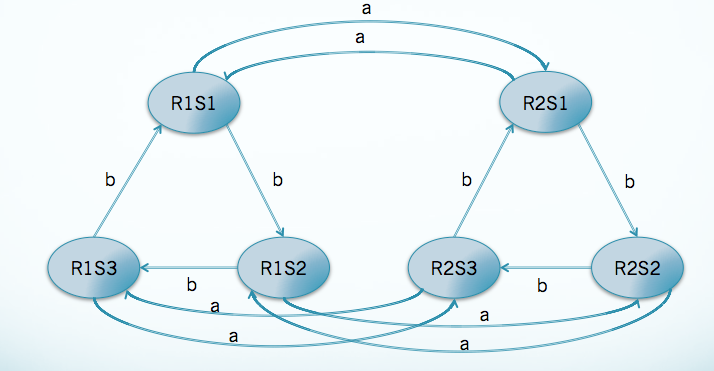
\includegraphics[width=12cm,height=7cm]{product.png}
\caption{Product of HMMs, P = R x S}
\label{fig:pohmm}
\end{figure*}

\section{Training Product of experts by minimising contrastive divergence}
High dimensional distributions are approximated as a product of one dimensional distributions. The product of individual distributions which is uniguassian or multivariate guassian will also be multivariate guassian. If the individual models are more complicated and contain one or more hidden variables, multiplying their distributions together and renormalizing them can be very powerful. These individual models are called "experts".
The product of experts produce sharper distribution than the individual distributions\cite{hinton2000}.

\section{Proof of concept on REDD House 2}
%\begin{enumerate}
\subsection{Aim}
 To represent streams of energy consumption data from $n$\footnote{n=2} appliances by product(s) of $k$ HMMs.
 
\subsection{Method} 

\begin{itemize}
\item \textbf{Data } The Reference Energy Disaggregation Data Set (REDD) is used in empirical analysis. The data contains power consumption from real homes, for the whole house as well as for each individual circuit in
the house (labeled by the main type of appliance on that circuit). It is intended for use in developing disaggregation methods, which can predict, from only the whole-home signal, which devices are being used. The REDD data set contains two main types of home electricity data: high-frequency current/voltage waveform data of the two power mains (as well as the voltage signal for a single phase), and lower-frequency power data including the mains and individual, labeled circuits in the house. The main directory consists of several house\_i directories, each of which contain all the power readings for a single house.  Each house subdirectory consists of a labels.dat and several channels\_i.dat files. The labels file contains channel numbers and a text label indicating the general category of device on this channel. Each channel\_i.dat file has two columns containing UTC timestamps (as integers) and power readings (recording the apparent power of the circuit) for the channel.
Experiments reported here use the House 2 data from REDD. It has $11$ channels where each channel corresponds to the following appliance: 
\begin{enumerate}
\item mains$\_1$ 
\item mains$\_2$ 
\item kitchen$\_$1
\item lighting
\item stove 
\item microwave
\item washer$\_$dryer
\item kitchen$\_2$
\item refrigerator
\item dishwaser
\item disposal
\end{enumerate}

The dataset has $318759$ records and $2$ columns. We randomly sample 300 records for our experiment. Time series data from two appliances are represented as product of $k$ HMMs.


\item \textbf{ Time Series :} The time series data of the microwave, dryer, kitchen$\_2$ and refrigerator are plotted below in Figures~\ref{fig:micro}, ~\ref{fig:washer}, ~\ref{fig:kitchen2}, ~\ref{fig:refri}.

\begin{figure*}[t]
\centering
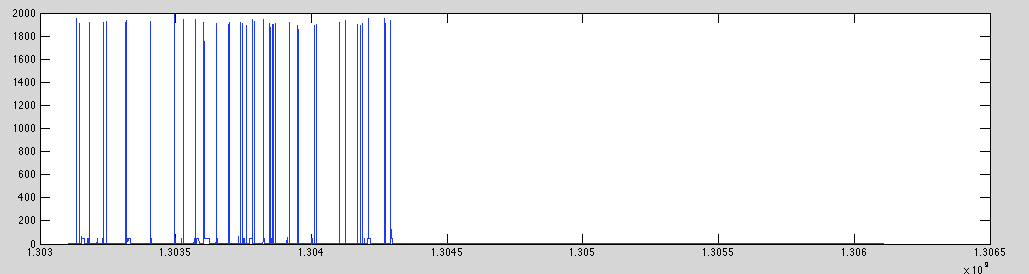
\includegraphics[width=1.0\textwidth,height=0.15\textheight]{channel_6.png}
\caption{Microwave}
\label{fig:micro}
\end{figure*}

\begin{figure*}[t]
\centering
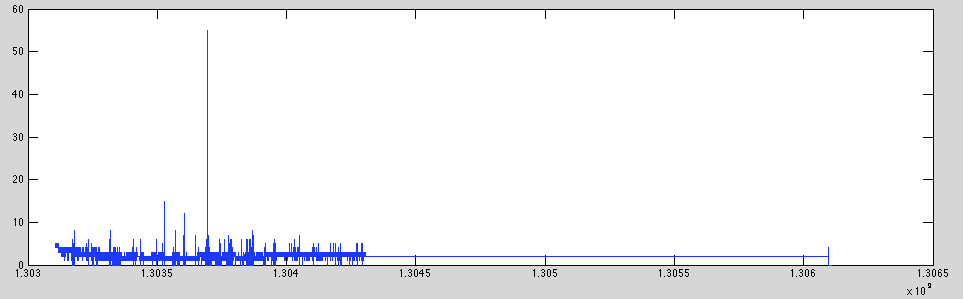
\includegraphics[width=1.0\textwidth,height=0.15\textheight]{channel_7.png}
\caption{washer\_dryer}
\label{fig:washer}
\end{figure*}

\begin{figure*}[th]
\centering
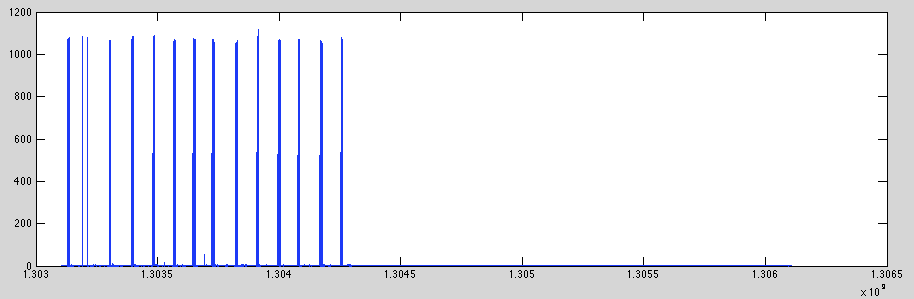
\includegraphics[width=1.0\textwidth,height=0.15\textheight]{channel_8.png}
\caption{Kitchen\_2}
\label{fig:kitchen2}
\end{figure*}

\begin{figure*}[th]
\centering
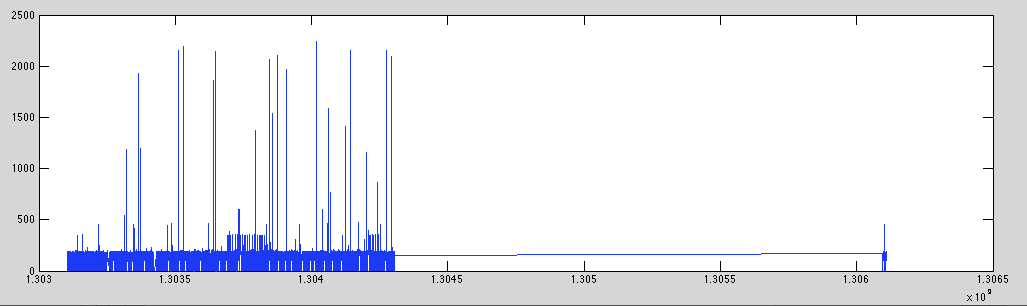
\includegraphics[width=1.0\textwidth,height=0.15\textheight]{channel_9.png}
\caption{refrigerator}
\label{fig:refri}
\end{figure*}

\item \textbf{Code } The implementation of the product of experts model is obtained from Iain Murray's website \cite{Iain}. It implements the technique described in Geoff Hinton's paper \cite{hinton2000}. 

\item \textbf{Additional details }
Some additional details regarding experiments:
\begin{enumerate}
\item The product of HMMs model (PoHMM) minimizes ``contrastive divergence" as described in the paper \cite{hinton2000}. 
\item The number of experts, $k$ used here is 15. This is set somewhat arbitrarily and needs to be experimented on.
\item Learning rate is $\epsilon = \frac{1}{300}$.
\end{enumerate}
 
\end{itemize}

\subsection{Results }
This section shows the graphs for different combinations of devices representing how well the learning by product of experts on real data takes place. Experts try to fit the generated data (fantasy data) to the means calculated from the real data. The results of the following pairwise appliances, microwave \& washer, Kitchen$\_$2 \& refrigerator and microwave \& refrigerator are plotted below in Figures~\ref{fig:img1}, ~\ref{fig:img2}, ~\ref{fig:img3}. The black dots represent the fantasy data that is generated from the product of experts. Mean computed by the real data is shown by red dots and ellipses in blue show the one standard deviation contours of the Gaussians in each expert.
There are 15 unigauss experts each of which is a mixture of a uniform and a single, axis aligned guassian. These experts are initialized with randomly located, circular gaussians that have the same variance as the data.
In the fitted model, each tight data cluster is represented by the intersection of two Gaussians which are elongated along different axes.

\begin{figure*}[th]
\centering
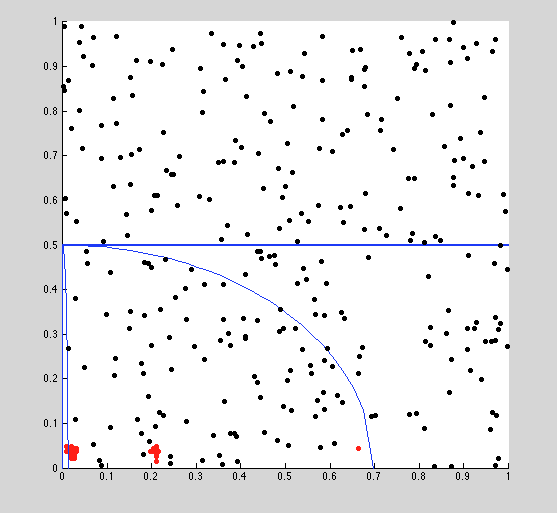
\includegraphics[width=14cm,height=6cm]{channel_6_7.png}
\caption{Training product of experts for microwave and washer$\_$dryer}
\label{fig:img1}
\end{figure*}

\begin{figure*}[th]
\centering
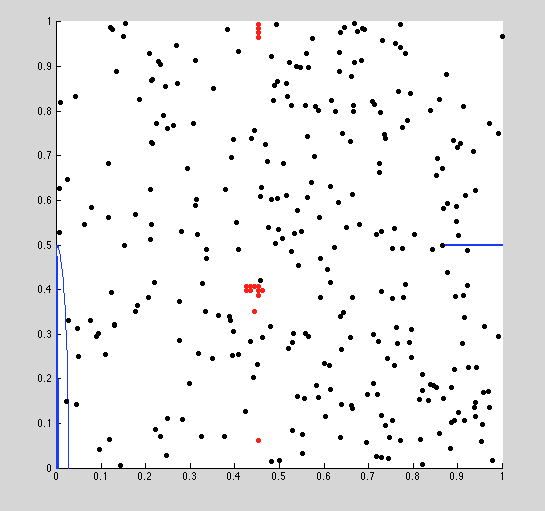
\includegraphics[width=14cm,height=6cm]{channel_8_9.png}
\caption{Training product of experts for Kitchen$\_2$ and refrigerator}
\label{fig:img2}
\end{figure*}

\begin{figure*}[th]
\centering
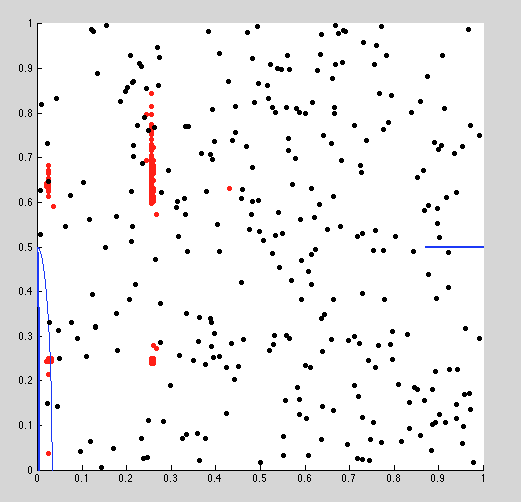
\includegraphics[width=14cm,height=6cm]{channel_6_9.png}
\caption{Training product of experts for microwave and refrigerator}
\label{fig:img3}
\end{figure*}

%\end{enumerate}


\bibliography{HMM_writeup}
\bibliographystyle{plain}


\end{document}